\subsection{Erstellung des Betriebssystem-Image}\label{sw_image}
Nach erfolgreichem Test des Installationsskripts\footnote{Siehe Abschnitt \ref{ah_skript}: \nameref{ah_skript}} haben wir für je einen Raspberry Pi 3 und einen Raspberry Pi 4 ein Image erstellt.
Hierzu haben wir mit Hilfe des Raspberry Pi Imagers eine 8 Gigabyte große Micro-SD-Karte\footnote{Zum Zeitpunkt der Erstellung des Images kleinstmögliche vorhandene Micro-SD-Karte} mit Raspberry Pi OS in der 32-Bit-Variante geflasht. 
Dieser kann über die Tastenkombination [STRG]+[SHIFT]+[X] die Grundeinstellungen wie SSH, Domänennamen und Passwort festlegen (vgl. \ref{fig:create_image_01}).
Dementsprechend wurden für die beiden Versionen folgende Einstellungen vorgenommen:\\
\begin{table}[H]
    \begin{tabularx}{\textwidth}{|p{3cm}|p{3cm}|p{4cm}|p{3.7cm}|}
        \hline
        \textbf{Image-Name} & \textbf{User} & \textbf{Passwort} & \textbf{Domänename} \\
        \hline
        \verb|shz_rp3.img.gz| & pi & raspberry & shzpi3\\
        \hline
        \verb|shz_rp4.img.gz| & pi & raspberry & shzpi4\\
        \hline
    \end{tabularx}
    \caption{Überblick über die Images für die Raspberry Pis}
    \label{tab:image_uebersicht}
\end{table}
\noindent Nachdem die Image auf die SD-Karte geflasht wurden, haben wir die Raspberry Pis mit den entsprechenden Karten bestückt und uns per SSH mit den Geräten verbunden.\\
\noindent Mit Hilfe des Shell-Befehls
\mint{bat}|ssh pi@<Domänenname>|
\noindent und der Verwendung des Standardpasswords haben wir uns mit den Raspberry Pis verbunden (vgl. Tab. \ref{tab:image_uebersicht}: \nameref{tab:image_uebersicht}.
Anschließend haben wir das Skript auf dem Pi eingerichtet und gestartet (vgl. \ref{fig:create_image_02}).
Nachdem das Skript ausgeführt wurde (vgl. \ref{fig:create_image_03}) wurde die SD-Karte mit Win32 Disk Imager in eine .img-Datei konvertiert (vgl. \ref{fig:create_image_04}).
Anschließend wurde die Image mit 7Zip komprimiert, um Speicherplatz zu sparen (vgl. \ref{fig:create_image_05}). Diese Images können dann mit dem Raspberry Pi Imager\footnote{Alternative: balnea Etcher} wieder auf SD-Karten geflasht werden.\\
\noindent Die Images\footnote{Stand: Ende März 2021} können über folgende Links heruntergeladen werden:
\begin{itemize}
    \item Raspberry Pi 3 Image: \url{https://www.mediafire.com/file/bc2o542na3rea7j/shz_rp3.img.gz/file}
    \item Raspberry Pi 4 Image: \url{https://www.mediafire.com/file/eujoh6s4thpg363/shz_rp4.img.gz/file}
\end{itemize}
\begin{figure}[H]
    \begin{subfigure}[b]{0.5\linewidth}
        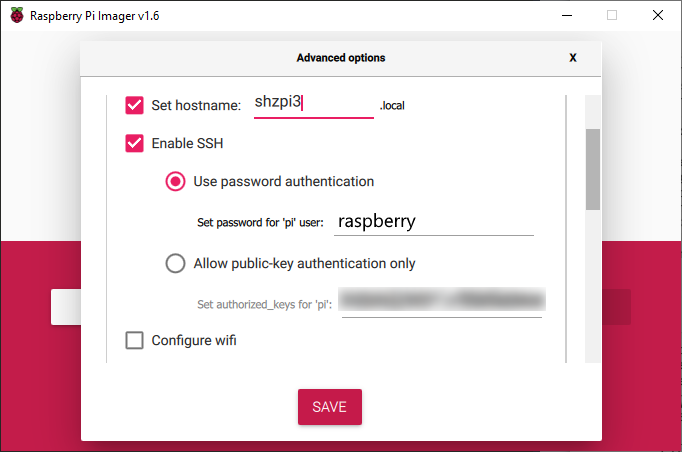
\includegraphics[width=1\textwidth]{img/pi_img_3_settings.png}
        \caption[Einstellungen des Raspberry Pi Imager]{Einstellungen des Raspberry Pi Imager}
        \label{fig:create_image_01}
    \end{subfigure}
    \begin{subfigure}[b]{0.5\linewidth}
        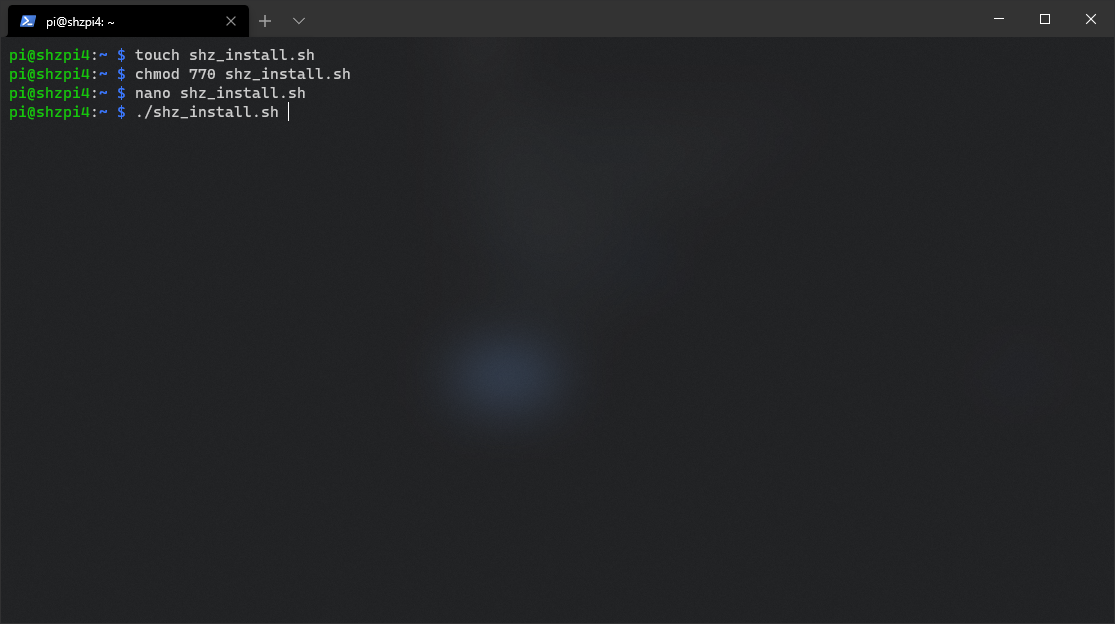
\includegraphics[width=1\textwidth]{img/pi_img_ssh.png}
        \caption[Durchgeführte Befehle auf Raspberry Pi]{Durchgeführte Befehle auf Raspberry Pi}
        \label{fig:create_image_02}
    \end{subfigure}
    \begin{subfigure}[b]{0.5\linewidth}
        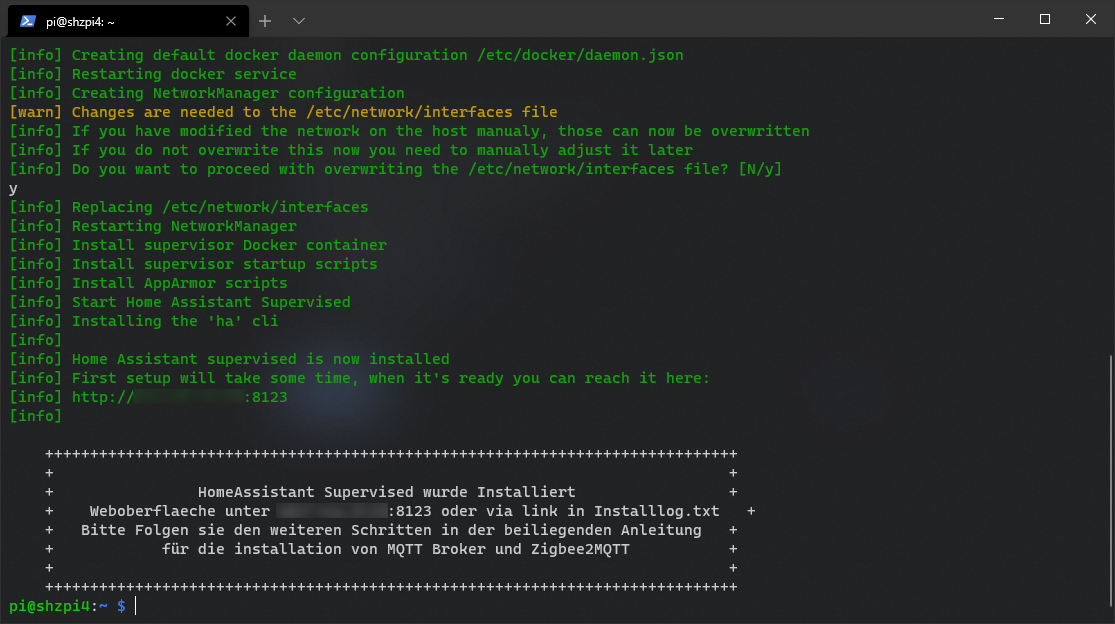
\includegraphics[width=1\textwidth]{img/pi_img_ssh_end.png}
        \caption[Letze Ausgabe des Pi]{Letzte Ausgabe des Pi}
        \label{fig:create_image_03}
    \end{subfigure}
    \begin{subfigure}[b]{0.5\linewidth}
        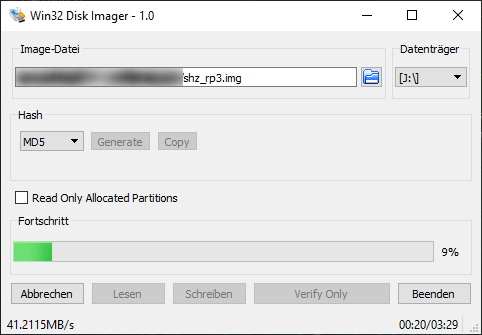
\includegraphics[width=1\textwidth]{img/pi_img_3_windiskimg.png}
        \caption[Erstellen des Images]{Erstellen des Images}
        \label{fig:create_image_04}
    \end{subfigure}
    \begin{subfigure}[b]{0.5\linewidth}
        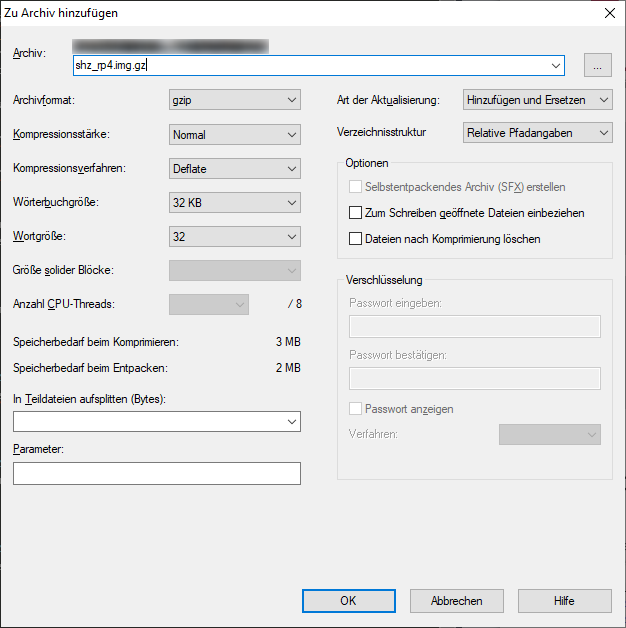
\includegraphics[width=1\textwidth]{img/pi_img_7zip.png}
        \caption[7Zip-Einstellungen]{7Zip-Einstellungen}
        \label{fig:create_image_05}
    \end{subfigure}
    \caption[Erstellen der Images]{Erstellen der Images}
    \label{fig:create_image}
\end{figure}
